\documentclass{article}

\usepackage{fancyhdr}
\usepackage{ragged2e}
\usepackage{graphicx}
\usepackage{caption}
\usepackage{geometry}
\usepackage{amsmath}
\usepackage{rotating}

\usepackage{listings}
\usepackage{color}

\definecolor{dkgreen}{rgb}{0,0.6,0}
\definecolor{gray}{rgb}{0.5,0.5,0.5}
\definecolor{mauve}{rgb}{0.58,0,0.82}

\lstset{frame=tb,
  language=Java,
  aboveskip=3mm,
  belowskip=3mm,
  showstringspaces=false,
  columns=flexible,
  basicstyle={\small\ttfamily},
  numbers=none,
  numberstyle=\tiny\color{gray},
  keywordstyle=\color{blue},
  commentstyle=\color{dkgreen},
  stringstyle=\color{mauve},
  breaklines=true,
  breakatwhitespace=true,
  tabsize=4
}

\setcounter{secnumdepth}{1}

\usepackage{chngcntr}
\counterwithin{figure}{section}

\renewcommand*{\thepage}{C\arabic{page}}

\pagestyle{fancy}
\lhead{ACME Robotics}
\chead{\#8367}
\rhead{\ifcontents Contents \else Week \thesection \fi}

\newif\ifcontents
\contentsfalse

\makeatletter
\renewcommand{\@seccntformat}[1]{}
\makeatother

\begin{document}

\subsection{Build and test the glyph lifter at the 24-hour build}
%!Assemble the main lifter mechanism and lifter/grabber at the 24-hour build.
At the 24 hour build, the Hardware Team's goal was to build a working lifter/grabber on a functional drive base. In the beginning, we drew sketches of potential lifter designs. Then, once we had a few ideas on a lifter mechanism shown in figure \ref{fig:brainstorm}, we started to test different lifters that we had sketched out. 
\begin{figure}[h]
    \centering
    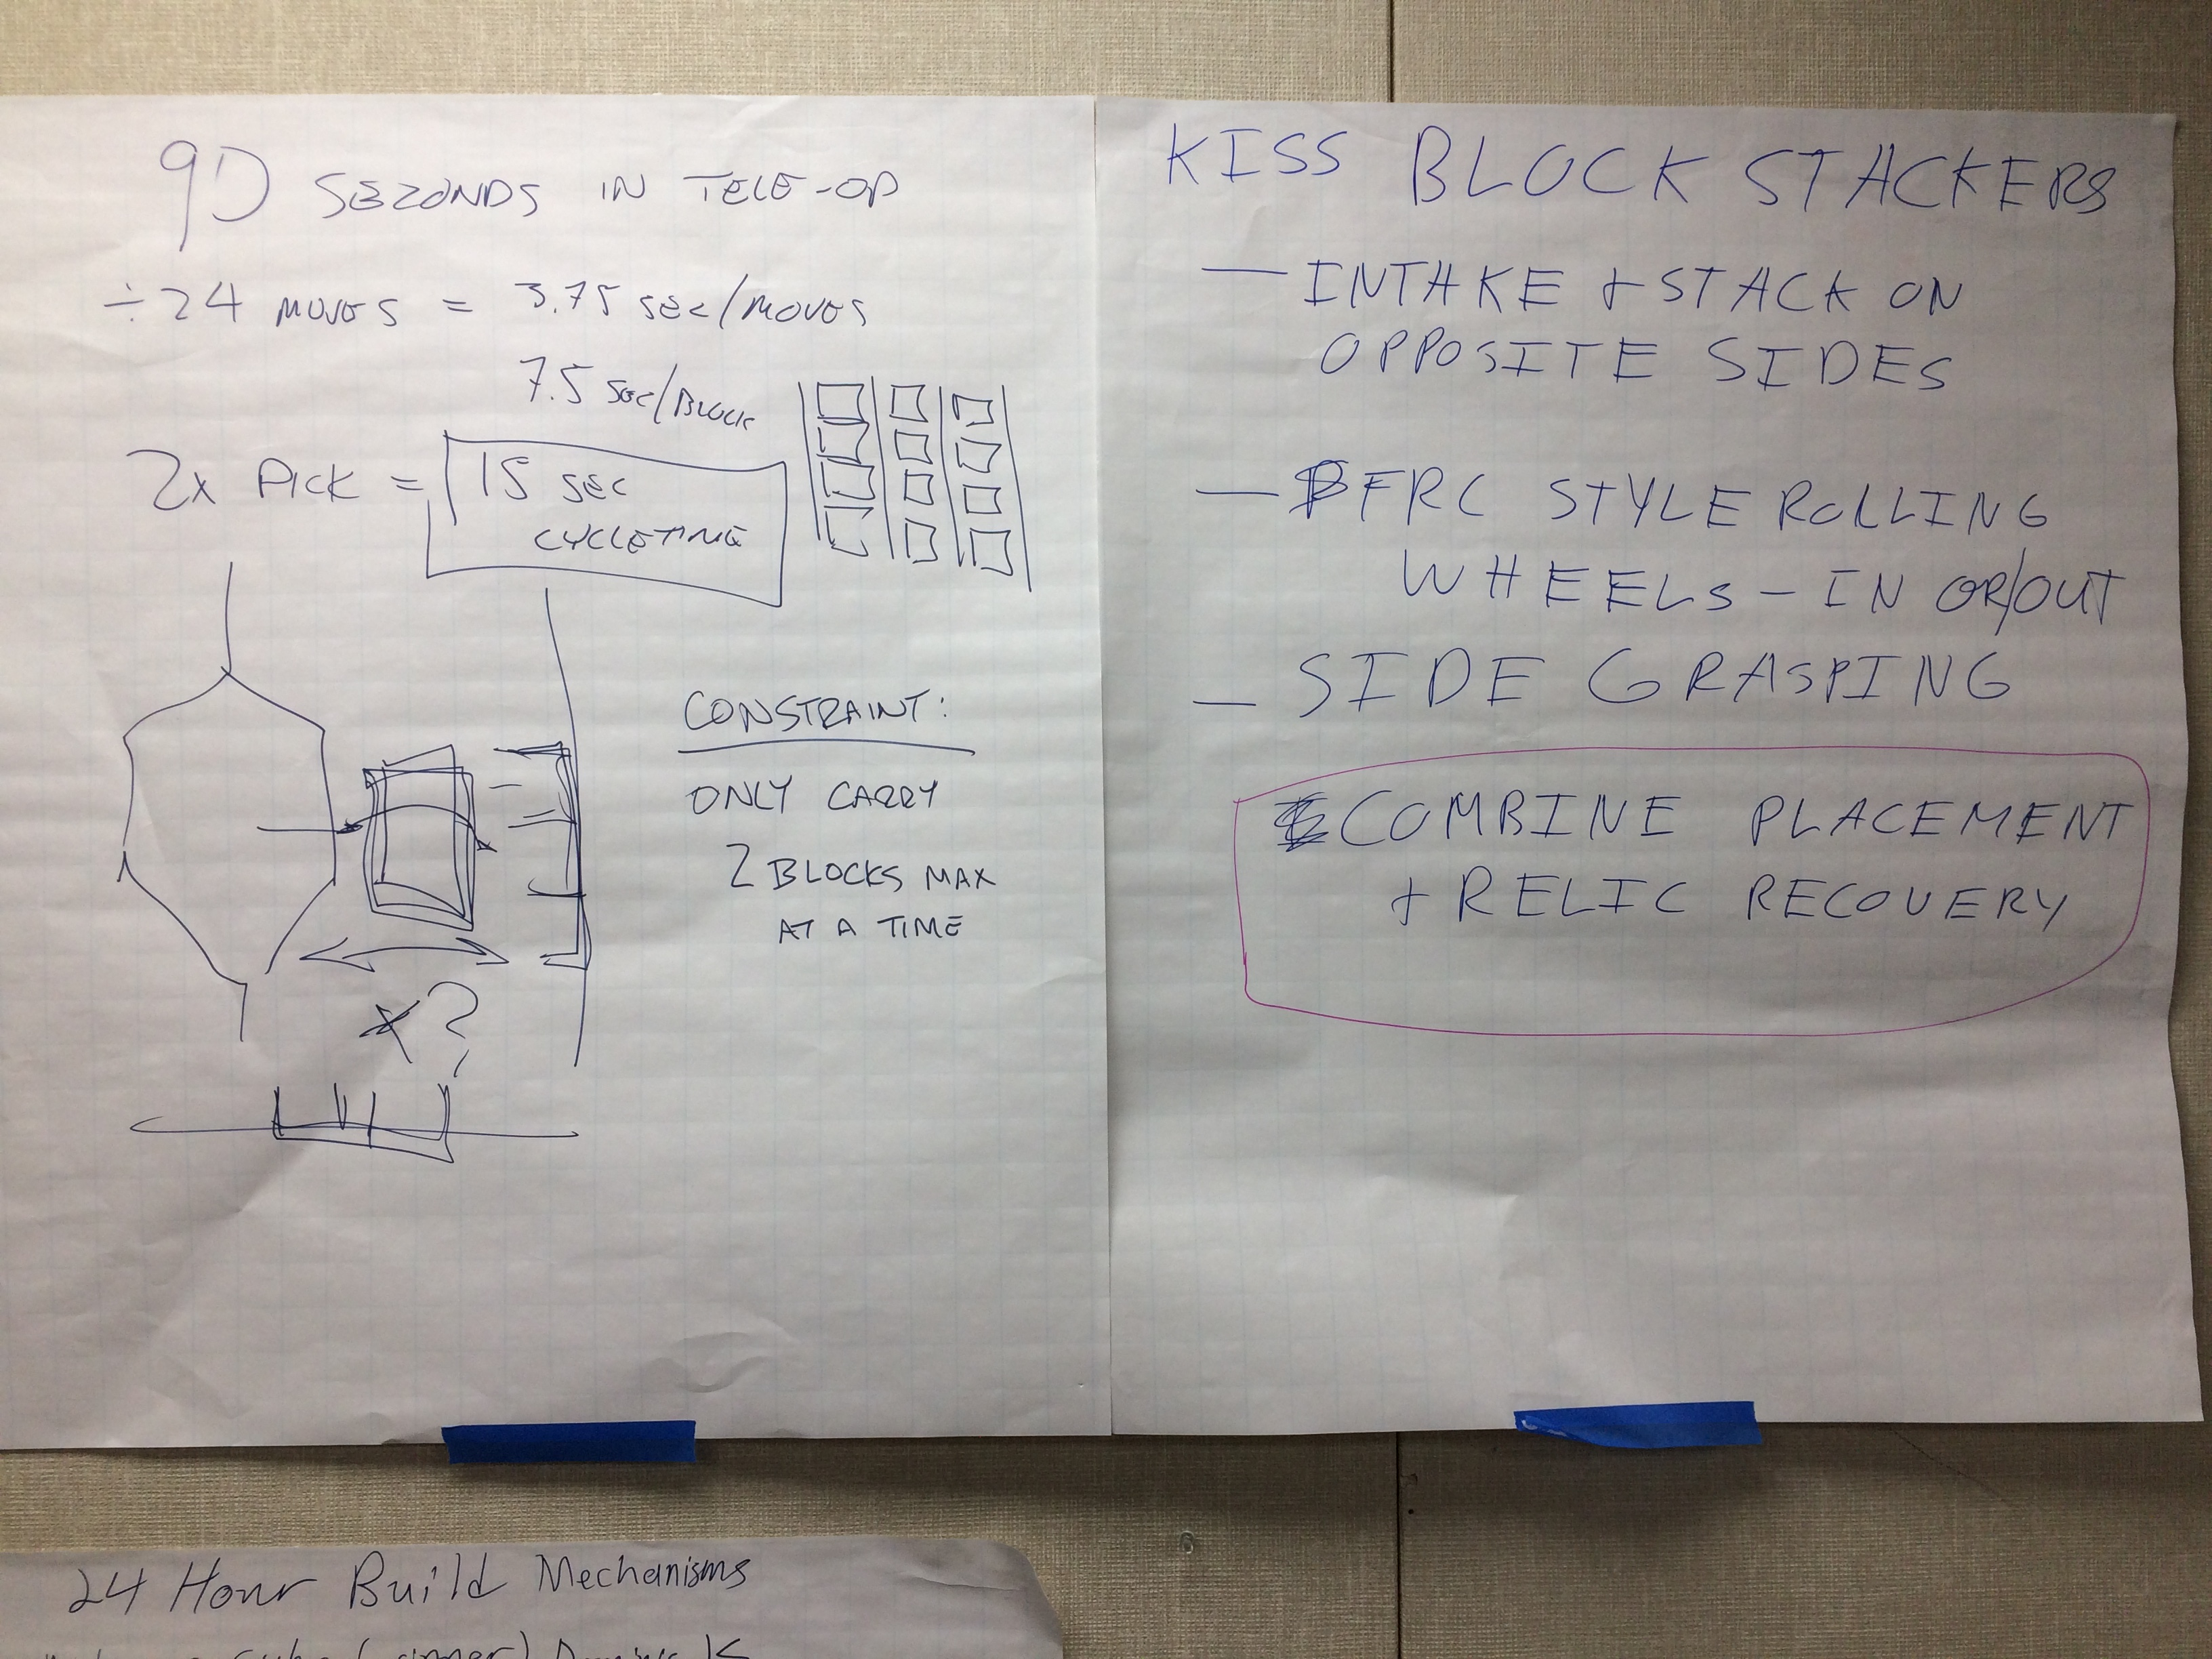
\includegraphics[width=.8\textwidth]{01/images/brainstorm.jpg}
    \caption{brainstormting}
    \label{fig:brainstorm}
\end{figure}
After testing the different ideas, our final decision was a parallel lift, driven on one side. We then started the building and assembly of the grabber. This took us a few hours to complete and put onto the drive base. We came across a few struggles, such as parts not cooperating, broken parts, and flaws in the design. This included the arm not being rigid enough, which was resolved by putting cross braces across the arm. The gears powering the arm were skipping, due to misalignment, but this was solved by the addition of shims and Zip Ties. In the end, we had a fully functional lifter, that can be seen in figure \ref{fig:robot}. We tested this mechanism, and it worked for the most part, other than us having to come up with a way to grip the glyphs and lift them up. 
\begin{figure}[h]
    \centering
    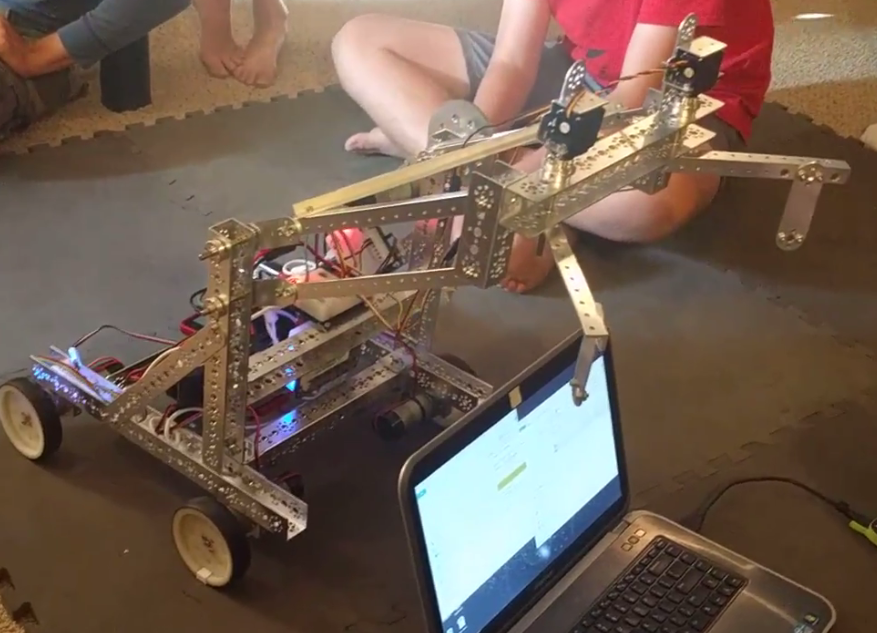
\includegraphics[width=.6\textwidth]{01/images/robot.png}
    \caption{robot}
    \label{fig:robot}
\end{figure}

\subsection{Build and test the linear slide}
%!Assemble the basic slide and then customize it to the correct size and bulk.
At the 24-hour build,  Ben was assigned the task of building the linear slide for the relic. He watched the REV linear motion kit how-to video and assembled the slide without difficulty. Then, our mentor Mike and Ben drew some sketches of our visions for the linear slide and how it was going to work. He decided on a design that allowed the slide to fit into the sizing cube and not take up a lot of bulk. Next, he put the metal stock into a vise and hack sawed them into 16 inch lengths. Finally, he assembled the slide according to the drawings. Also, he had to add WD-40 to make the mechanism slide smoother. He also made some sketches of the slide before he started cutting things. Figure \ref{fig:sketch} shows the sketch that Ben and Mike made before they cut the extrusion.
\begin{figure}[h]
    \centering
    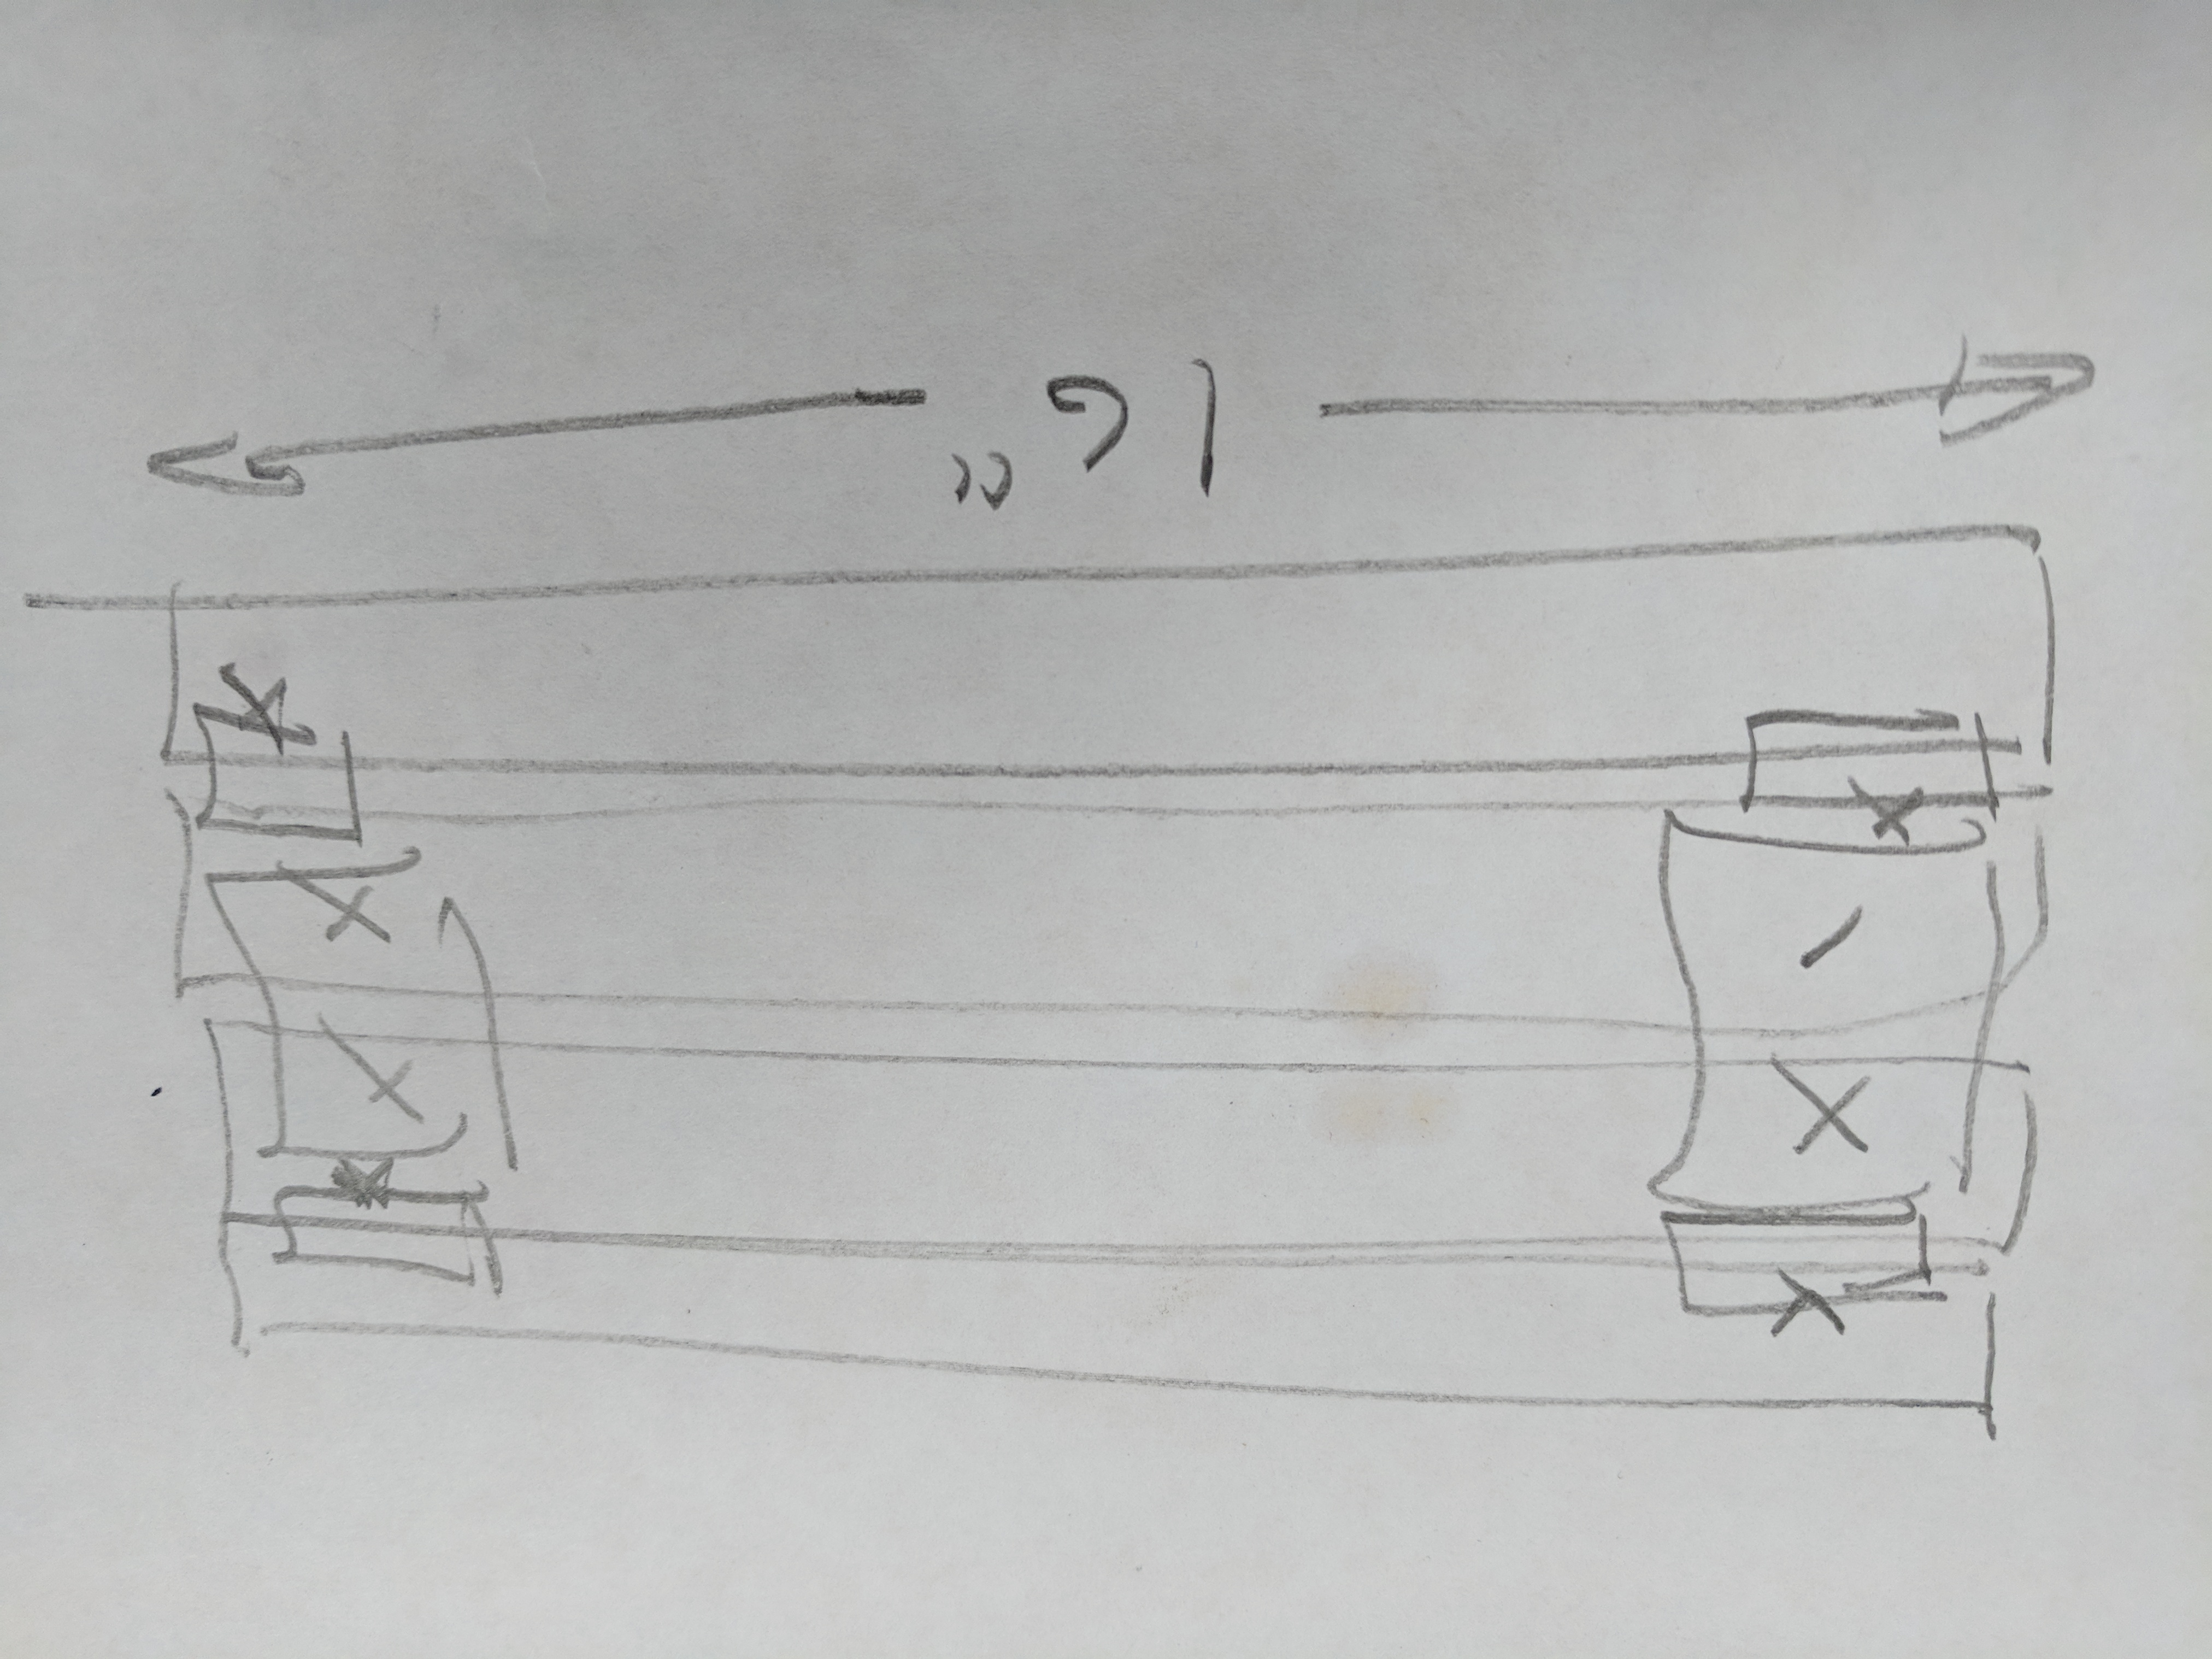
\includegraphics[width=.6\textwidth]{01/images/Sketch2.jpg}
    \caption{sketch}
    \label{fig:sketch}
\end{figure}

\subsection{Build and test drive base}
%!The goal for the drive base is to create a platform on which the mechanisms can be mounted and tested. The requirements are that it has to have either two or four wheel drive, as well as a place to mount the phone, battery, and modules.
For the 24 hour build, we needed a drive base to attach whatever mechanisms we made to in order to test them properly. We had a test base already built to test the REV module, with phone and battery mounts as well as four motors and wheels. We decided to modify this base instead of building a new one around the mechanism because it was less time consuming and worked just as well. In order for the mechanism to work, we replaced the small tetrix wheels on the base with larger ones, moved the motors inwards, away from the corners, and moved the position of the modules. In the end, the drive base functioned perfectly and allowed us to test all the modules we wanted.

\end{document}